\documentclass[11pt]{article}
\usepackage[a4paper,margin=1in]{geometry}
\usepackage{enumitem}
\usepackage{hyperref}
\usepackage{amsmath}
\usepackage{pgfplots}
\usepackage{booktabs}
\usepackage{longtable}
\usepackage{array}

\pgfplotsset{compat=1.18}

\title{Mental Math Progression \& Level System (v1)}
\author{Christian Köhler}
\date{}

\begin{document}

\maketitle

\section{Long term goal}

The long-term vision for the mental math application is to provide a highly personalized,
adaptive training experience.
The system is structured around independent mathematical domains,
each featuring a progressive ladder of calculation patterns.

\begin{itemize}[leftmargin=*]
    \item \textbf{Level-based training}: Each level corresponds to a specific pattern of calculations to master.
    \item \textbf{Domain-specific ladders}: User progress is tracked independently per domain, meaning each domain has its own level ladder.
    \item \textbf{Personalized progression}: Advancement is tailored to the user and evaluated based on two primary factors:
    \begin{itemize}
        \item Correctness: Whether the calculation was solved correctly.
        \item Speed: How fast the calculation was solved compared to other users.
    \end{itemize}
    \item \textbf{Comprehensive domains}: The full system will eventually support a wide range of operations:
    \begin{itemize}
        \item Addition
        \item Subtraction
        \item Multiplication
        \item Division
        \item Root
        \item Square
        \item Power
    \end{itemize}
    \item \textbf{Adjustable difficulty}: Users can manually tune their difficulty level (e.g., warm up, normal, hard).
    \item \textbf{Customizability}: Training configurations will include toggles to allow for negative numbers (minus) and decimals.
\end{itemize}

\section{Version 1}

Version 1 establishes the core mechanics. It is a simplified version of the long-term goal with the following constraints:

\begin{itemize}[leftmargin=*]
    \item \textbf{Limited domains}: Only Addition, Subtraction, Multiplication, and Division will be available.
    \item \textbf{Fixed difficulty parameters}: There will be no difficulty settings (warm up, normal, hard) to choose from. Time cutoffs for correct solves will be hard-coded rather than percentile-based.
    \item \textbf{No customizability}: Calculations will exclusively feature positive numbers and no decimals.
\end{itemize}

\subsection{Pattern-Based Levels}

Each domain (Addition, Subtraction, Multiplication, Division) is divided into ten progressive levels.
A \textbf{pattern} specifies the constraints for the questions generated at that level.

\subsubsection*{Generation Rules}

To ensure an appropriate and consistent learning curve, all patterns adhere to the following global rules:

\begin{itemize}[leftmargin=*]
  \item \textbf{Positive Results Only}: Subtraction questions never yield negative numbers.
  \item \textbf{Exact Division}: All division questions result in exact integers, with no remainders.
  \item \textbf{Meaningful Divisions}: Both divisors and quotients are always $\ge 2$ to prevent trivial cases (like $n \div 1$ or $n \div n$).
  \item \textbf{Meaningful Multiplications}: Multiplication operands are always $\ge 2$ to prevent trivial cases (like $n \times 1$).
  \item \textbf{Operand Order Randomization}: For commutative operations (Addition and Multiplication) with differing digit lengths, the display order is randomized (e.g., a 1-digit and 2-digit addition can appear as $17+2$ or $2+17$).
\end{itemize}

\subsubsection*{Progression Tables}

The domain ladders are defined in the tables below based on the following metrics:

\begin{itemize}[leftmargin=*]
  \item \textbf{Level} --- Sequential difficulty step within each domain (1 = easiest).
  \item \textbf{Operands} --- The number of digits per operand (e.g., $2 \times 1$ means a 2-digit number and a 1-digit number).
  \item \textbf{Complexity (Carries / Borrows / Quotient)} --- The operations required to solve the calculation. For Addition, Subtraction, and Multiplication, this refers to the exact number of carries or borrows. For Division, this indicates the number of digits in the resulting \textbf{quotient}.
  \item \textbf{Cutoff (ms)} --- Minimum time budget per question to achieve a ``solved'' status in v1.
\end{itemize}

\vspace{1em}

\noindent
\begin{minipage}[t]{0.48\textwidth}
\subsubsection*{Addition (ADD)}
\begin{center}
\begin{tabular}{@{}lccc@{}}
\toprule
\textbf{Level} & \textbf{Operands} & \textbf{Carries} & \textbf{Cutoff (ms)} \\
\midrule
1  & $1 + 1$ & 0 & 4\,000 \\
2  & $1 + 1$ & 1 & 4\,000 \\
3  & $1 + 2$ & 0 & 4\,500 \\
4  & $1 + 2$ & 1 & 4\,500 \\
5  & $2 + 2$ & 0 & 5\,000 \\
6  & $2 + 2$ & 1 & 5\,000 \\
7  & $2 + 2$ & 2 & 5\,500 \\
8  & $2 + 3$ & 0 & 5\,500 \\
9  & $2 + 3$ & 1 & 6\,000 \\
10 & $3 + 3$ & 0 & 6\,000 \\
\bottomrule
\end{tabular}
\end{center}
\end{minipage}
\hfill
\begin{minipage}[t]{0.48\textwidth}
\subsubsection*{Subtraction (SUB)}
\begin{center}
\begin{tabular}{@{}lccc@{}}
\toprule
\textbf{Level} & \textbf{Operands} & \textbf{Borrows} & \textbf{Cutoff (ms)} \\
\midrule
1  & $1 - 1$ & 0 & 4\,000 \\
2  & $2 - 1$ & 0 & 4\,500 \\
3  & $2 - 1$ & 1 & 4\,500 \\
4  & $2 - 2$ & 0 & 5\,000 \\
5  & $2 - 2$ & 1 & 5\,000 \\
6  & $3 - 1$ & 0 & 5\,000 \\
7  & $3 - 1$ & 1 & 5\,500 \\
8  & $3 - 2$ & 0 & 5\,500 \\
9  & $3 - 2$ & 1 & 6\,000 \\
10 & $3 - 3$ & 0 & 6\,000 \\
\bottomrule
\end{tabular}
\end{center}
\end{minipage}

\vspace{2em}

\noindent
\begin{minipage}[t]{0.48\textwidth}
\subsubsection*{Multiplication (MUL)}
\begin{center}
\begin{tabular}{@{}lccc@{}}
\toprule
\textbf{Level} & \textbf{Operands} & \textbf{Carries} & \textbf{Cutoff (ms)} \\
\midrule
1  & $1 \times 1$ & 0 & 4\,000 \\
2  & $1 \times 1$ & 1 & 4\,000 \\
3  & $1 \times 2$ & 0 & 4\,500 \\
4  & $1 \times 2$ & 1 & 4\,500 \\
5  & $1 \times 2$ & 2 & 5\,000 \\
6  & $1 \times 3$ & 0 & 5\,000 \\
7  & $1 \times 3$ & 1 & 5\,500 \\
8  & $1 \times 3$ & 2 & 5\,500 \\
9  & $1 \times 3$ & 3 & 6\,000 \\
10 & $2 \times 2$ & 0 & 6\,000 \\
\bottomrule
\end{tabular}
\end{center}
\end{minipage}
\hfill
\begin{minipage}[t]{0.48\textwidth}
\subsubsection*{Division (DIV)}
\begin{center}
\begin{tabular}{@{}lccc@{}}
\toprule
\textbf{Level} & \textbf{Operands} & \textbf{Quotient} & \textbf{Cutoff (ms)} \\
\midrule
1  & $1 \div 1$ & 1 & 4\,000 \\
2  & $2 \div 1$ & 1 & 4\,000 \\
3  & $2 \div 1$ & 2 & 4\,500 \\
4  & $2 \div 2$ & 1 & 5\,000 \\
5  & $3 \div 1$ & 2 & 5\,500 \\
6  & $3 \div 1$ & 3 & 6\,000 \\
7  & $3 \div 2$ & 1 & 6\,500 \\
8  & $3 \div 2$ & 2 & 7\,000 \\
9  & $4 \div 2$ & 2 & 7\,500 \\
10 & $4 \div 2$ & 3 & 8\,000 \\
\bottomrule
\end{tabular}
\end{center}
\end{minipage}

\subsection{Progression Rules (v1: Hard-Coded Cutoff)}

User progression through the levels of a given domain is evaluated based on recent performance. For version 1, each level has a hard-coded \textbf{cutoff time} $C_L$ (which may later be replaced by population percentiles).

An attempt is considered \textbf{solved} if the correct answer is submitted first try and within $C_L$ milliseconds. Otherwise, the attempt counts as \textbf{unsolved}.

\subsubsection*{Promotion}

To advance from the current level $L$ to $L + 1$, the user must demonstrate consistent mastery. The system evaluates the last $N$ completed attempts at Level $L$:
\[
N = 5
\]
Promotion requires that \textbf{all} of the last $N$ attempts are solved. Once this condition is satisfied, Level $L + 1$ is unlocked.

\subsubsection*{Demotion}

To prevent users from being stuck on a level that is too difficult, the system employs a demotion rule based on the last $M$ attempts at the current level:
\[
M = 10
\]
A user is demoted if the unsolved rate over these $M$ attempts exceeds a maximum tolerance $S_{max}$:
\[
S_{max} = 0.25 \quad (25\%)
\]
Demotion is only allowed after a minimum exposure of $M$ attempts at that level.

\textbf{Soft Demotion:} Demotion is intentionally soft. If the user is at level $L$, a demotion moves them to $L-1$ (with a minimum level of $1$). This applies even if the triggering failures happened on a sampled lower-level question $k < L$. For example, if a user at level $10$ repeatedly fails sampled level $8$ questions, their new level is $9$, not $7$.

Formally:

\[
L_{new} = \max(1, L - 1)
\]

\subsection{Level Selection During Play}

The system dynamically samples question levels during play to balance current level mastery with review of previous levels and introduction of the next level.
The sampling algorithm is heavily weighted towards the user's current level,
with a fixed probability for the next level and a geometrically decaying probability for all lower levels.

\subsubsection*{Symbol Definitions}

Before detailing the selection mechanism, the following variables are defined:
\begin{itemize}[leftmargin=*]
    \item $L$: current user level in the domain
    \item $k$: sampled question level
    \item $r \in (0,1)$: geometric decay factor for lower levels (smaller $r$ means faster taper)
    \item $u(k)$: unnormalized geometric weight for lower levels
\end{itemize}

\subsubsection*{Sampling Formula}

During play, the next question level $k$ is drawn from the set of available levels up to a slight stretch goal:
\[
k \in \{1,2,\dots,L,L+1\}
\]

The probability mass is statically distributed to the upper levels:
\[
p(L)=0.50, \qquad p(L+1)=0.10
\]

The remaining mass is allocated to all lower levels ($1$ to $L-1$):
\[
\sum_{k=1}^{L-1} p(k)=0.40
\]

This $0.40$ is distributed over levels $1..L-1$ using a geometric taper so that levels closer to $L$ are more probable:
\[
u(k)=r^{(L-1)-k}, \qquad 1 \le k \le L-1
\]
\[
p(k)=0.40\cdot\frac{u(k)}{\sum_{j=1}^{L-1} u(j)}, \qquad 1 \le k \le L-1
\]

In the case where the user is at the first level ($L=1$), the distribution simplifies to:
\[
p(1)=0.90, \qquad p(2)=0.10
\]

Therefore, the current level maintains the highest probability, the next level is fixed at $10\%$, and all previous levels are sampled with decreasing probability.


\subsubsection*{Example Distribution}

As an example, assuming a user is at level $L=4$ with a decay factor $r=0.6$, the resulting probabilities $p(k)$ taper off logarithmically for the lower levels:

\begin{center}
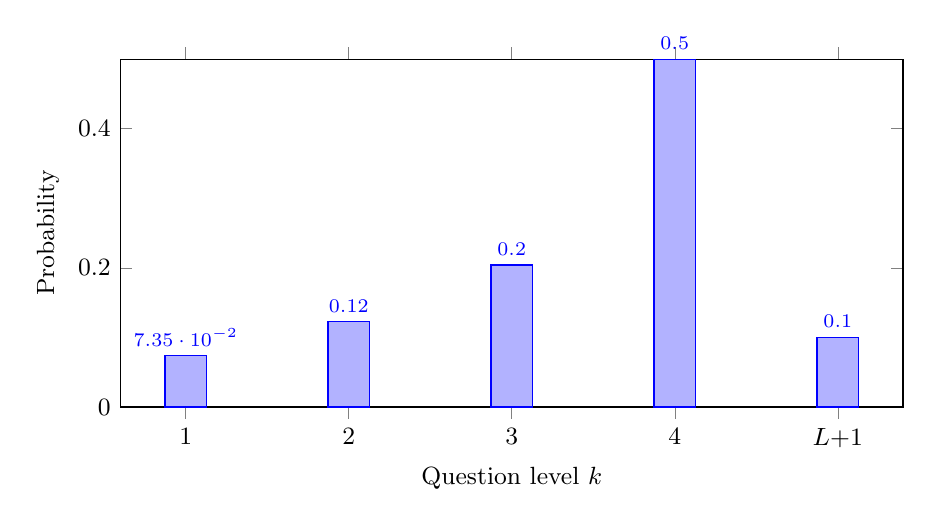
\begin{tikzpicture}
\begin{axis}[
    ybar,
    width=0.95\linewidth,
    height=6.0cm,
    ymin=0,
    ymax=0.5,
    ylabel={Probability},
    xlabel={Question level $k$},
    xtick={1,2,3,4,5},
    xticklabels={1,2,3,4,$L{+}1$},
    bar width=15pt,
    enlarge x limits=0.1,
    nodes near coords,
    nodes near coords align={vertical},
    every node near coord/.append style={font=\scriptsize},
    tick label style={font=\small},
    label style={font=\small}
]
\addplot coordinates {
    (1,0.0735)
    (2,0.1224)
    (3,0.2041)
    (4,0.5000)
    (5,0.1000)
};
\end{axis}
\end{tikzpicture}
\end{center}

\subsection{How Questions are stored}

\begin{enumerate}[leftmargin=*]
    \item Store \textbf{Pattern} rows (the generator rules).
    \item Generate question instances on demand using a RNG seed.
    \item Store each user interaction as an \textbf{Attempt} row.
\end{enumerate}

So, in practice, the ``question'' is represented by:

\begin{center}
\texttt{(patternId, seed)}
\end{center}

\subsubsection*{How a Pattern is stored in DB}

Each pattern family is one row in the \texttt{pattern} table.

Stable, indexed fields are stored as normal columns:

\begin{itemize}[leftmargin=*]
        \item \texttt{id}: unique pattern id
        \item \texttt{domain}: \texttt{ADD | MUL | SUB | DIV}
        \item \texttt{level}: ladder level within domain
        \item \texttt{description}: human-readable pattern label
        \item \texttt{cutoffTimeMs}: solved-time cutoff for v1
        \item \texttt{active}: enable/disable pattern
        \item \texttt{createdAt}, \texttt{updatedAt}: audit timestamps
\end{itemize}

Dynamic generation constraints are stored in:

\begin{itemize}[leftmargin=*]
        \item \texttt{params} (Prisma \texttt{Json}, PostgreSQL \texttt{JSONB})
\end{itemize}

Uniqueness rule in v1:

\begin{center}
\texttt{UNIQUE(domain, level, description)}
\end{center}

\subsubsection*{What \texttt{params} JSON looks like}

In v1, digit fields are stored as single integers (not lists),
because each pattern uses one fixed digit size per side.

\textbf{ADD example (Level 3: 1-digit + 2-digit, no carry)}

\begin{verbatim}
{
    "operation": "ADD",
    "leftDigits": 1,
    "rightDigits": 2,
    "carryCount": 0
}
\end{verbatim}

\textbf{MUL example (Level 5: 1-digit x 2-digit, two carries)}

\begin{verbatim}
{
    "operation": "MUL",
    "leftDigits": 1,
    "rightDigits": 2,
    "carryCount": 2
}
\end{verbatim}

\textbf{SUB example (Level 5: 2-digit - 2-digit, single borrow)}

\begin{verbatim}
{
    "operation": "SUB",
    "leftDigits": 2,
    "rightDigits": 2,
    "borrowCount": 1,
    "allowNegative": false
}
\end{verbatim}

\textbf{DIV example (Level 3: 2-digit / 2-digit, exact integer)}

\begin{verbatim}
{
    "operation": "DIV",
    "dividendDigits": 2,
    "divisorDigits": 2,
    "exactInteger": true,
    "minQuotient": 2
}
\end{verbatim}
\end{document}

